\documentclass{article}
\usepackage{pack}
\usepackage[backend = bibtex, sorting = none]{biblatex}
\addbibresource{main.bib}

\title{Rapport de soutenance à mi-parcours}
\author{Balthazar Charles}

\begin{document}
	\maketitle
	
	\abstract{Ce rapport de soutenance à mi-parcours présente les travaux de thèse effectués au mois d'avril 2021. Cette thèse, "Matrices de Cartan modulaires des monoïdes finis" a pour objectif en premier lieu de mettre en place des algorithmes permettant le calcul explicite de matrices de Cartan en exploitant des propriétés combinatoires des monoïdes, et en deuxième lieu de démarrer une exploration assistée par le calcul formel de la combinatoire de ces matrices, et en particulier de mettre en relief des parallèles entre le cas modulaire des monoïdes et les cas mieux connus non modulaire pour les monoïdes et modulaire pour les groupes.
	
	Après un rappel du contexte théorique dans lequel se situe la thèse, on rappelle son sujet, puis on  introduit les notions nécessaires. On décrit ensuite brièvement les travaux effectués à date : un algorithme pour calculer des points fixes dans un monoïde fini et une formule accompagnée d'un algorithme pour calculer la table de caractères d'un monoïde. L'accent est mis sur la description du premier algorithme, qui nécessite moins de notions théoriques que le second. On discute ensuite les travaux prévus et restants à effectuer sur le sujet de thèse, dont en particulier une publication en cours de préparation. Le dernier point de ce rapport concerne un sujet de recherche secondaire, sur les groupes de Coxeter qui a donné lieu a une publication et présente des perspectives intéressantes.}
	
	\newpage
	
	\section*{English summary}
	
	This document is a summary of the progression of the PhD work on the subject "Modular Cartan matrices of finite monoids" as of April 2021. 
	The investigations presented here stem from the developement over the last two decades of an interest for the combinatorics of monoid representations that arose from the seminal article \cite{Brown.2000} where Brown establishes a connection between the representation of certain kinds of monoids and some discreet Markov used the randomly generate conbinatorial objects. This thesis can be understood as a continuation of the results in \cite{AyyerSchillingSteinbergThiery.2014.RTrivivalMarkovChains}, \cite{AyyerSchillingThiery.2014.SpectralGap} and specially \cite{Thiery.CartanMatrixMonoid} where Thiéry gives a description of the Cartan matrix.
	
	More precisely, the object of this thesis is to use the formula given by Thiéry to design a (mostly) combinatorial algorithm to compute Cartan matrices and then to use it to take an exploratory approach to the combinatorics of  monoid representations. This computationnal exploration is motivated by the example of the full transformation monoid $T_n$ with the objective of revealing some parallels of its better understood group analogous, $\symm_n$.
	
	Thiéry's formula for the Cartan matrix of a monoid $M$ involves two main components : computing, for $h, k \in M$, the cardinality of $\{s \in M \sep hsk = s\}$, and computing the character table of $M$. Both of these tasks raise some challenges. We present the result of our investigations in the Section \href{sec:travaux}{\emph{Travaux}} and briefly summarize them below.
	\begin{itemize}
		\item The difficulty with counting fixed points is with the cardinality of the monoids: we have $|T_n| = n^n$, making brute force counting impractical even in small cases. In the first subsection of \href{sec:travaux}{\emph{Travaux}} we describe an algorithm to efficiently compute  the number of fixed points: on a particular $\hc$-class $H$, the two elements $h, k$ acts "as group elements" or "as zero" and this action can be factorized along the $\lc$ and $\rc$-classes containing $H$.
		\item For the second point, it is, in general, not straightforward to compute de the character table of a monoid (although some results are known, see \cite[Section 9.4]{steinberg2016representation}). In the second subsection of \href{sec:travaux}{\emph{Travaux}}, we present a decomposition of regular $\lc$-classes. We use this decomposition to compute the character table of the monoid. The resulting algorithm reuses the fixed points counting method developed in the previous point, but combinatorial methods are not enough and part of the algorithm relies on solving a linear system.
	\end{itemize}

	More work is required: firstly, the resolution of the linear system is, as of now, the limiting factor in the computation as it involves $\sim 10^6$ equations in $\sim10^6$ variables for $T_8$. This can be mitigated using specialized algorithms for sparse linear system, and further reductions exploiting the structure of the monoid should be investigated in the near future.
	Secondly, although the case of representation on fields of null characteristic is already implemented, group radical computation are not yet integrated in the modular case.
	Finally, most of the exploratory work remains to be done. For now, we have a formula for the Cartan Matrix of $T_n$ in null characteristic, but due to the implementation of the modular case algorithm being incomplete we have yet to explore the positive characteristic case.
	
	Finally, we briefly discuss an secondary line of research on Coxeter groups, which lead to a publication \cite{Baba2020} on a conjecture from Dyer \& Hohlweg in \cite{dyer2016small}. In addition to further research on this subject, this helped to launch an ongoing collaboration with some students from LaCIM, Montreal, about some algorithmic aspects of Coxeter groups.
	
	\newpage
	
	\section*{Contexte}
	
	Les objets centraux de cette thèse sont les \emph{monoïdes finis}, 
	que l'on peut voir comme des groupes finis l'axiome d'inversibilité 
	en moins, et leurs \emph{représentations}.
	
	\begin{dftn}
		Un \emph{monoïde} est un ensemble $M$, muni d'une loi de 
		composition associative pour laquelle il existe un élément neutre. 

		Une \emph{représentation} d'un monoïde fini $M$ est la donnée d'un
		corps $\kbf$, d'un espace vectoriel de dimension finie $V$ et d'une
		structure de $\kbf M$-module sur $V$.
	\end{dftn}
	
	La théorie des représentations des monoïdes est a priori beaucoup plus
	difficile que la théorie des représentations des groupes. En particulier, 
	alors que toutes les représentations de groupes finis peuvent être 
	décomposées en sommes directes de \emph{représentations irréductibles} 
	(c'est-à-dire engendrées par n'importe quel élément non nul en tant que 
	$\kbf M$-modules), ce n'est pas le cas des représentations de monoïdes. 
	On dit que l'algèbre $\kbf M$ du monoïde n'est pas \emph{semi-simple}. 
	La \emph{matrice de Cartan} est, dans un sens, une statistique qui 
	mesure le défaut de semi-simplicité de $\kbf M$.
	
	Comme dans le cas des groupes, la théorie des \emph{caractères} (le 
	caractère d'une représentation $V$, noté $\chi_V$, étant définit comme 
	l'application qui à $m \in M$ associe la trace de la multiplication par 
	$m$ vue comme endomorphisme de $V$), joue un rôle important dans l'étude 
	des représentations des monoïdes.
	Dans \cite{Thiery.CartanMatrixMonoid}, Thiéry donne une formule pour calculer 
	la matrice de Cartan à partir de la table de caractères du monoïde $X_M$ et 
	du caractère de l'algèbre $\kbf M$ elle-même vue comme une représentation de 
	$M$, et qui peut être définie en termes de comptage de point fixes. On peut 
	se servir de cette formule comme définition de la matrice de Cartan. Plus 
	précisément :
	
	\begin{dftn}\label{def:cartan}
		Soit $\mathcal{V}$ un ensemble de représentants des classes d'isomorphisme 
		de représentations irréductibles de $M$ pour un corps $\kbf$ et $C_M$ un 
		sous ensemble maximal de $M$ tel que pour tout $m, m' \in C_M$, $m \neq m' 
		\Rightarrow \chi_V(m)\neq \chi_V(m')$ pour un certain $V \in \mathcal{V}$. 
		La \emph{table de caractères} est la matrice carrée :
		\[X_M = (\chi_V(m))_{V \in \mathcal{V}, m \in C_M},\]
		le \emph{bicaractère} de $\kbf M$ la matrice carrée :
		\[B = (|\{s \in M \sep msm' = s\}|)_{m, m' \in C_M},\]
		et finalement, la \emph{matrice de Cartan} est la matrice carrée :
		\[C(\kbf M) = X_M B X_M^T.\]
	\end{dftn}
	
	\section*{Sujet}
	
	La présente thèse s'inscrit dans une dynamique d'étude des représentations 
	des monoïdes finis au cours des deux dernières décennies, suite à l'article précurseur~\cite{Brown.2000} du fait d'applications aux chaînes de Markov 
	discrètes; notamment celles utilisées pour tirer aléatoirement des objets 
	combinatoires. Dans la lignée de ces travaux, cette thèse a pour but de 
	mettre en place des outils informatiques et algorithmiques pour explorer la 
	combinatoire des représentations des monoïdes révélée dans des articles tels 
	que \cite{Brown.2000,AyyerSchillingSteinbergThiery.2014.RTrivivalMarkovChains,AyyerSchillingThiery.2014.SpectralGap}, dans le cadre plus général des monoïdes finis sur un
	corps (presque) quelconque.
	
	Plus particulièrement, on peut noter que dans la définition précédente, la 
	matrice de Cartan dépend du corps car la table de caractères dépend du corps.
	L'objet de la thèse est donc de \emph{mettre en place des outils permettant de 
	calculer efficacement la matrice de Cartan d'un monoïde fini sur un corps de 
	caractéristique quelconque}. Un tel outil permettrait une approche 
	exploratoire de la combinatoire des représentations de certains monoïdes.
	
	En particulier, cette recherche est motivée par l'étude de la famille des 
	monoïdes $T_n$ de toutes les transformations d'un ensemble de taille $n$, 
	et en particulier la détermination de la matrice de Cartan de $T_n$ dans 
	le cas modulaire. Cette famille est l'analogue dans la théorie des monoïdes 
	de la famille des groupes symétriques $S_n$, dont la théorie des représentations, modulaire comme non-modulaire, est régie par une belle combinatoire 
	(partitions, tableaux, ...). Les résultats 	existants confirment qu'il y a 
	tout lieu de penser que le même phénomène a lieu pour $T_n$.
	
	\section*{Travaux}\label{sec:travaux}
	
	Dans cette section, on présente succinctement les résultats obtenus jusqu'ici. Pour cela, on introduit dans une première partie quelques notions de théorie des monoïdes et de leur représentations avant de présenter les travaux réalisés dans une seconde.
	
	\subsection*{\'Eléments de théorie des monoïdes et de leurs représentations}
	
	Dans un monoïde où on n'a pas l'axiome d'inversibilité d'un groupe, la question de savoir si un élément est un multiple d'un autre devient non triviale. Comme les monoïdes considérés sont en général non commutatifs, la notion de multiple doit être déclinée : ainsi, deux éléments $m, m$ d'un monoïde $M$ sont en $\lc$-relation s'ils ont le même ensemble de multiples à gauche, en $\rc$-relation s'ils ont les mêmes multiples à droite et en $\jc$-relation pour les multiples des deux côtés. $\lc, \rc$ et $\jc$, auxquelles on ajoute la $\hc$-relation définie par $m\hc m' \Leftrightarrow m\rc m'$ et $m\lc m'$ sont les \emph{relations de Green}.
	
	\begin{lined}
		\begin{ex}[Relations de Green dans $T_3$]
			La loi du monoïde est la composition des fonctions.
		
			{\centering
			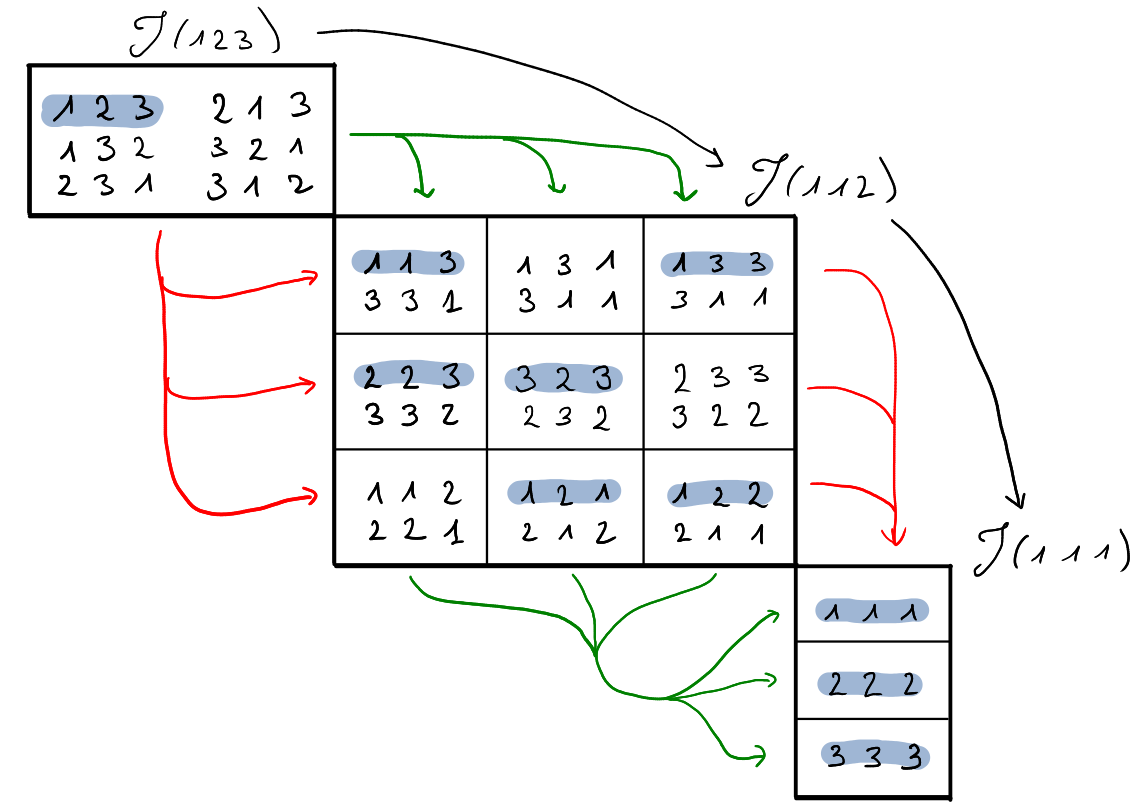
\includegraphics[width=0.95\textwidth]{./ordres.png}}
			
			Les éléments sont notés par les uplets représentant leurs valeurs. Les $\jc$-classes sont les blocs, les $\lc$-classes les colonnes et les $\rc$-classes sont les lignes. Les $\hc$-classes sont les cases aux intersections des $\lc$ et $\rc$-classes. Les relations de couverture de $\jc, \lc$ et $\rc$-ordres sont représenté en noir, rouge et vert respectivement. Les éléments surlignés sont les \emph{idempotents} : ils vérifient $e^2 = e$.
		\end{ex}
	\end{lined}
	
	Sur l'exemple précédent on peut voir que les $\jc$-classes se décomposent proprement en union de $\lc$ et $\rc$ classes : c'est l'image en "boîte à \oe{}ufs\footnote{C'est le terme consacré.}". C'est un fait général et une conséquence de l'important lemme suivant.
	
	\begin{lemme}[Lemme de Green]
		Soient $R, R'$ deux $\rc$-classes de la même $\jc$-classe, et soient $a \in R$ et $a' \in R' \cap \lc(a)$. Soient $\lambda, \lambda'$ tels que $\lambda a = a'$ et $\lambda' a' = a$. Les applications $x \mapsto \lambda x$ et $x \mapsto \lambda$ sont des bijections inverses l'une de l'autre entre $R$ et $R'$, mais aussi entre $R \cap \lc(a)$ et $R' \cap \lc(a)$.
	\end{lemme}

	On a évidemment un énoncé similaire pour la multiplication à droite. 
	
	\begin{lined}
		\begin{ex}[$\jc$-classe de $1,1,2$ dans $T_3$]
		On regarde ici l'effet de la composition à gauche par $2,1,3$ et à droite par $2,3,2$.
		
		{\centering
		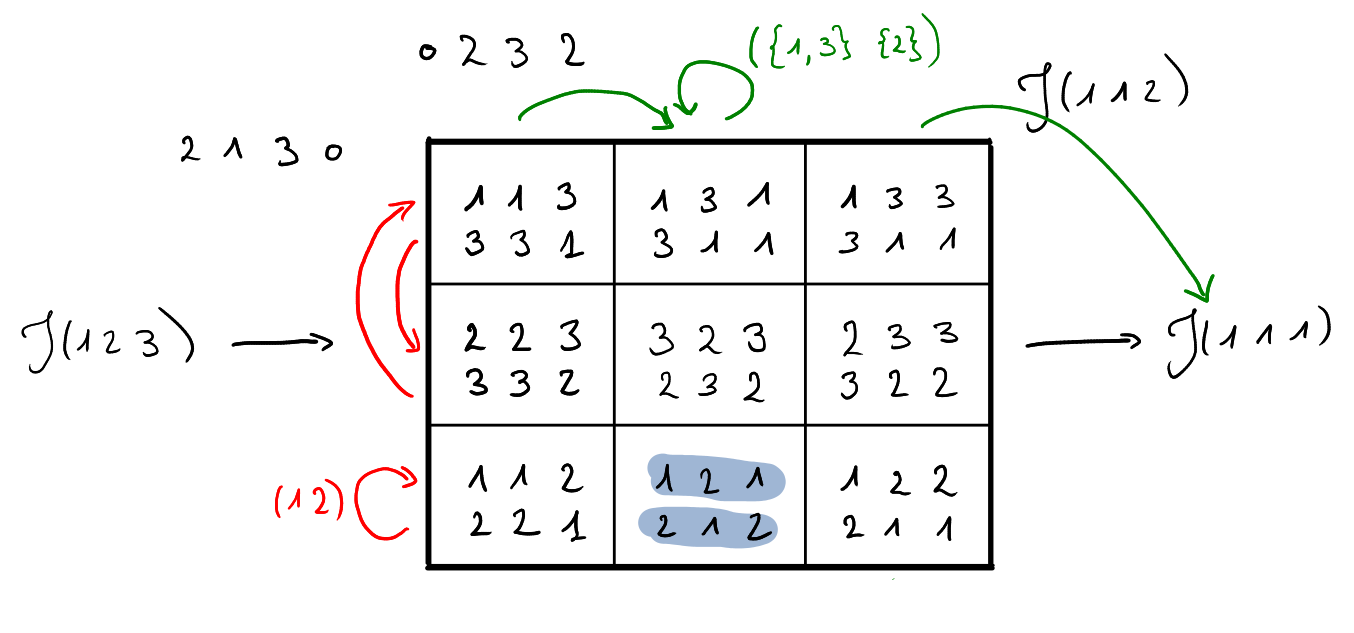
\includegraphics[width=0.95\textwidth]{./green.png}}
	
		La composition à gauche par $2,1,3$ stabilise seulement $\rc(1, 2, 1)$ et agit sur $\rc(1, 2, 1)$ comme la composition par la transposition $(1\ 2)$.
		La composition à droite par $2, 3, 2$ stabilise seulement $\lc(1, 2, 1)$ et fait descendre $\lc(1, 2, 2)$ dans une $\jc$-classe $\jc$-inférieure. Cette composition agit sur $\lc(1, 2, 1)$ comme la composition par la transposition $(\{1, 3\}\ \{2\})$. Les points fixés par les deux compositions appliquées simultanément sont indiqués en bleu.
		\end{ex}
	\end{lined}

	Une conséquence du lemme de Green est que si la multiplication à gauche par un élément du monoïde stabilise une $\hc$-classe $H$ donnée, alors c'est en fait une permutation de $H$. L'ensemble des permutations de $H$ obtenu de cette façon est le \emph{groupe de \schu} à gauche de $H$, noté $\Gamma(H)$. De la même façon, on définit le groupe de \schu à droite $\Gamma'(H)$. Ce groupe encode, d'une certaine façon, une information redondante sur la $\jc$-classe de $H$ : $\Gamma(H)$ et $\Gamma(H')$ sont isomorphes si $H, H'$ sont dans la même $\jc$-classe. On a la même chose pour $\Gamma'$ et de plus, pour tout $H$, $\Gamma(H)$ et $\Gamma'(H)$ sont anti-isomorphes. Ces (anti-)isomorphismes ne sont en général pas canoniques, mais sont faciles à calculer.
	
	\begin{lined}
		\begin{ex}[$\jc$-classe de $1,1,2$ dans $T_3$]\label{ex:green}
			Les groupes de \schu gauches et droits des $\hc$-classes de $\jc(1,1,2)$ sont tous isomorphes à $\symm_2$. L'isomorphisme entre $\hc(1,1,3)$ et $\hc(2,2,3)$ est simplement la composition à gauche par $(2,1,3)$.
		\end{ex}
	\end{lined}
	
	On peut noter dans l'exemple précédent que quand une $\hc$-classe $H$ contient un idempotent $e$, $H$ est un groupe de neutre $e$ naturellement isomorphe a ses groupes de \schu. C'est un fait général qui est utilisé dans le théorème fondamental suivant pour ramener la théorie de représentations des monoïdes finis à celle des groupes finis.
	
	\begin{thm}[Munn-Clifford-Ponizovskii]\label{thm:MCP}
		Soit $\jc_{reg}$ l'ensemble des $\jc$-classes contenant un idempotent et soit $\mathcal{E}$ un ensemble de représentants idempotents de $\jc_{reg}$.
		Pour $e \in \mathcal{E}$, notons $G_e = \hc(e)$. Pour un $\kbf M$-module $W$, notons également $N_e(W) = \{x \in \kbf W\sep eMx = 0 \}$
		Il y a une bijection entre les représentations irréductibles de $M$ sur $\kbf$ et celles des $G_e$ sur $\kbf$ donnée par :
		\[V^{\#} = \kbf \lc(e)\otimes_{\kbf G_e} V / N_e(\kbf \lc(e)\otimes_{\kbf G_e} V)\]
		$e$ étant un élément de $\mathcal{E}$ et $V$ une représentation irréductible de $G_e$ sur $\kbf$.
	\end{thm}
	
	On pourra consulter le cours de Jean-\'Eric Pin "Mathematical Foundations of Automata Theory" \cite{Pin:Automata} ainsi que le livre de Benjamin Steinberg \cite{steinberg2016representation} pour plus de détails.
	
	\subsection*{Résultats}
	
	Utiliser la formule de Thiéry pour calculer la matrice de Cartan présente deux difficultés. 
	\begin{enumerate}
		\item La première difficulté vient du fait que le cardinal de nombreuses familles intéressantes de monoïdes croit très rapidement. Par exemple, le cardinal de $T_n$ vaut $n^n$. 
		Pour résoudre ce problème, nous avons mis au point un algorithme permettant de calculer efficacement le cardinal de l'ensemble $\fix_J(h, k) = \{j \in J \sep hjk=j\}$ pour une $\jc$-classe $J$ et des éléments quelconque du monoïde $M$.
		\item Deuxièmement, calculer la table de caractères du monoïde est en soit une difficulté. Des résultats sont connus pour certaines classes de monoïdes \cite[Section 9.4]{steinberg2016representation}, mais la question de calculer la table de caractères d'un monoïde arbitraire est inexplorée dans un cas général.
		Pour résoudre ce problème, nous avons démontré une formule sur les caractères des monoïdes qui permet de réutiliser les méthodes de comptages de points fixes précédemment développées pour calculer la table de caractère d'une façon largement (mais pas seulement) combinatoire.
	\end{enumerate}
	
	
	\paragraph{1 - Compter des points fixes}
	
	Grace au lemme de Green, on voit que si $hsk = s$, alors $h$ stabilise $\rc(s)$ et $k$ stabilise $\lc(s)$, on peut donc interpréter $h, k$ comme des éléments de $\Gamma(\hc(s))$ et $\Gamma'(\hc(s))$, respectivement. Par ailleurs, bien que l'on ait mentionné que les (anti-)isomorphismes entre les groupes de \schu gauches et droits ne sont pas canoniques, on peut montrer que les classes de conjugaison de tous les $\Gamma(H), \Gamma'(H)$ pour $H$ parcourant les $\hc$-classes d'une $\jc$-classe sont en bijection canonique. On peut en dériver la propriété suivante :
	\begin{prop}
		Soit $h, s, k \in M$ tels que $hsk=s$. Alors $h, k$, vu comme éléments de $\Gamma(\hc(s))$ et $\Gamma'(\hc(s))$ sont dans "la même classe de conjugaison" et il y a cardinal du centralisateur de $h$ points fixés par $x \mapsto hxk$ dans $\hc(s)$.
	\end{prop}
	
	On en déduit un algorithme pour calculer les points fixes de l'application $x \mapsto hxk$ dans une $\jc$-classe $J$. Notons simplement $G$ un groupe de \schu d'une des $\hc$-classe de $J$. Pour une paire $h, k$ donnée on procède de la façon suivante :
	\begin{enumerate}
		\item Pour chaque classe de conjugaison $c$ de $G$, intialiser $r_c, l_c = 0$.
		\item Pour chaque $\rc$-classe $R$ contenue dans $J$, vérifier si $x \mapsto hx$ stabilise $R$, et si oui, calculer la classe de conjugaison $c$ correspondante et incrémenter $r_c$ de 1.
		\item Pour chaque $\lc$-classe $L$ contenue dans $J$, vérifier si $x \mapsto xk$ stabilise $L$, et si oui, calculer la classe de conjugaison $c$ correspondante et incrémenter $l_c$ de 1.
		\item Renvoyer $\sum_c r_cl_c\cdot |\textrm{centralisateur de }c|$
	\end{enumerate} 

	On pourra noter qu'on peut tabuler la première étape pour pouvoir calculer les points fixes pour différentes paires $(h, k_i)$ on ne faisant le calcul qu'un fois pour $h$, par exemple. En itérant cet algorithme sur toutes les $\jc$-classes, on peut calculer les points fixes dans le monoïde en entier, ce qui permet de calculer la matrice $B$ de la définition $\ref{def:cartan}$. En restreignant les étapes 2 et 3 on peut, par exemple, calculer les points fixes dans une $\rc$ ou $\lc$-classe donnée.
	
	Un brève analyse la complexité de cet algorithme donne, en notant $n_r$ et $n_l$ le nombre de $\rc$ et $\lc$-classes dans $\jc$, et $n_c$ le nombre de classe de conjugaisons de $G$ :
	\begin{itemize}
		\item $n_r + n_l$ tests d'appartenance à une $\lc$ ou $\rc$-classe,
		\item $O(n_r + n_l)$ calculs de classes de conjugaisons,
		\item $n_c$ calculs de cardinaux de centralisateurs et sommes.
	\end{itemize}
	Sans rentrer dans le détail des coûts spécifiques de chaque opération pour un monoïde général, une fois calculée une "bonne" structure de données pour le monoïde (voir \cite{east2019computing}) ces opérations peuvent être effectuées efficacement. Dans le cas spécifique du monoïde $T_n$, chacune des opérations peut être réalisée en $O(n)$, ce qui donne un $O(n(n_r+n_l+n_c))$.
	Il faut comparer cela au fait que dans la $\jc$-classe $J_k$ de $T_n$ dont tous les éléments ont une image de cardinal $k$, on a :
	\[|G| = k!, n_r = {n \choose k}, n_l = O\left(\frac{k^n}{k!}\right)\]
	avec une complexité de l'algorithme naif $O(n|G|n_rn_l)$ où le $n$ vient de la complexité de la multiplication de $T_n$.
	
	Cet algorithme est \textbf{déjà implémenté} dans le langage GAP et utilisé non seulement pour la formule donnant la matrice de Cartan, mais aussi pour des calculs intermédiaires pour trouver la table de caractères dans la partie suivante. 
	
	On peut noter que ces avancées ont été impulsées grâce à James D. Mitchell, à l'occasion de sa visite au LRI en février 2020.
	
	\paragraph{2 - Calculer la table de caractères}
	
	En partant du théorème de Munn-Clifford-Ponizovskii, on peut démontrer la relation suivante qui nous permet de calculer les caractères irréductibles du monoïde.
	
	\begin{prop}
		Soit $e \in M$ un idempotent et $G_e$ sa $\hc$-classe. Pour une représentation irréductible de $G_e$ sur $\kbf$, on note $V^{\#}$ la représenation correspondante par le théorème \ref{thm:MCP}. On a :
		\[\kbf\lc(e)/(\rad_{\kbf G_e}(\lc(e)) + N_e(\kbf \lc(e))) = \bigoplus_V V^{\#}\otimes V^*\]
		où $V$ parcourt les représentation irréductibles de $G_e$ et $\rad_{\kbf G_e}(\lc(e))$ est le radical de $\kbf \lc(e)$ en tant de $\kbf G_e$-module.
	\end{prop}
	
	Cette relation implique en particulier que si on connaît (i) le caractère de $\kbf \lc(e)$ et (ii) celui de $\rad_{\kbf G_e}(\lc(e)) + N_e(\kbf \lc(e))$, et qu'on connaît (iii) la table de caractère de $G_e$, alors on connaît les lignes de la table de caractères de $M$ associée à $G_e$.
	Le point (iii) relève de la théorie des représentations des groupes, et on considère ici que c'est une donnée du problème. Le point (i) peut-être obtenu efficacement par des méthodes de comptage de points fixes comme dans la précédemment. La difficulté réside dans (ii): le calcul du caractère de $\rad_{\kbf G_e}(\lc(e)) + N_e(\kbf \lc(e))$. Celui-ci n'a a priori pas de raison d'avoir une description combinatoire. Cette difficulté se décline de deux façons :
	
	\begin{itemize}
		\item Dans le cas où la caractéristique de $\kbf$ \emph{ne divise pas} $|G_e|$, cette somme se réduit à $N_e(\kbf \lc(e))$. En exploitant certains résultats sur la structure de Green de $\jc(e)$, on arrive à une description de cet espace par $|G_e|n_l$ équations à $|G_e|n_r$ inconnues. On peut ensuite en calculer une base puis le caractère.
		\item Dans le cas où la caractéristique de $\kbf$ divise $|G_e|$ (cas modulaire), il faut en plus $\rad_{\kbf G_e}(\lc(e))$. Cela est essentiellement équivalent à calculer le radical de l'algèbre $\kbf G_e$. Malheureusement, ce problème, bien que largement étudié (voir par exemple \cite{karpilovsky1987jacobson}), reste peu compris et difficile. En particulier, dans le cas de $T_n$, ces groupes sont des groupes symétriques, pour lesquels on dispose de peu de technologie en dehors d'algorithmes généralistes en $O(|G|^3)$ 
	\end{itemize}
	
	Grâce à cette formule on a pu calculer la table de caractère puis la matrice de Cartan de $T_n$ sur $\CC$ en utilisant la formule de Thiéry jusqu'à $n = 7$ en quelques secondes avec une implémentation GAP alors que des algorithmes généralistes implémentés dans Sagemath nécessitent plusieurs minutes de calcul pour $T_4$.
	
	\section*{Perspectives}
	
	Il y a deux types de perspectives sur le sujet de thèse : premièrement, du travail reste à faire sur le calcul effectif des matrices de Cartan et deuxièmement, une fois ces algorithmes en place une phase de "mathématiques expérimentales" est à envisager.
	
	Dans la première catégorie, la partie identifiée du travail restant est :
	\begin{itemize}
		\item Rendre plus efficace le calcul de l'opérateur $N_e$ : pour le moment, et même avec l'exploitation actuelle de la structure de Green, on est amené à résoudre une système linéaire de $\sim 10^6$ équations à $\sim 10^6$ inconnues dans le cas de $T_8$. Ces matrices sont très creuses et on peut envisager utiliser des méthodes de calculs adaptées en plus d'exploiter davantage les propriétés de la multiplication du monoïde.
		\item Rendre plus efficace le calcul du radical de l'algèbre du groupe dans le cas modulaire : pour le moment on utilise un algorithme pour une algèbre quelconque de dimension finie et le remplacer par un algorithme adapté aux algèbres de groupes permettrait de mener les calculs plus loin.
		\item Rendre disponible le code terminé pour le système de calcul formel GAP.
	\end{itemize}

	Dans la catégorie "mathématiques expérimentales", le travail à effectuer est plus difficile à identifier. Une fois les algorithmes finalement mis en place, le calcul de nombreux exemples pourrait permettre la mise à jour de motifs dans la matrice de Cartan que ce soit dans le cas modulaire ou non. On peut noter que le code traitant le cas non modulaire, qui est essentiellement achevé, a déjà permis de trouver une façon de calculer la matrice de Cartan de $T_n$ sur $\CC$ uniquement combinatoire, ne mettant en jeu que des tableaux d'Young. L'analyse de cette formule et de ses avatars en termes de fonction symétriques a pour le moment été laissée de côté, mais il est prévu d'y revenir.
	
	Enfin, les travaux déjà effectués présentés plus haut devraient faire l'objet d'une publication actuellement en cours de rédaction.
	
		\section*{Travaux supplémentaires}
	
	Dans le cadre d'un projet de recherche secondaire sur les groupes de Coxeter, un abstract étendu \cite{Baba2020} a été soumis à la conférence FPSAC (Formal Power Series and Algebraic Combinatorics) qui est (pour l'instant) prévue pour la semaine du 5 au 9 juillet à l'université Bar-Ilan en Israël. Le papier a été accepté pour une session de poster et est à paraitre dans les comptes rendus du Séminaire Lotharingien de Combinatoire 2021. On y annonce une preuve d'un cas particulier de la Conjecture 2 de \cite{dyer2016small}. Cet  abstract étendu a vocation à évoluer vers un article détaillé. 
	
	Ce travail de recherche trouve deux continuations naturelles : premièrement, il s'agirait d'appliquer ce résultat partiel comme lemme pour attaquer le cas général. Deuxièmement, un groupe de travail a été mis en place pour travailler sur la conjecture et des objets apparentés et en particulier sur la recherche d'algorithmes permettant de calculer et de générer combinatoirement ces objets. Ce groupe de travail est constitué en collaboration avec, en particulier, Nathan Chapelier-Laget du LaCIM à Montréal. Les perspectives de recherche sur ce projet secondaire s'ajoutent à celles précédemment évoquées concernant le sujet de thèse lui-même.
	
	\clearpage
	
	\section*{Références bibliographiques}
	
	\printbibliography
	
\end{document}